\documentclass[presentation]{beamer}

\usepackage{tikz}
\usetikzlibrary{positioning,calc}
\usetikzlibrary{shapes.geometric}
\usetikzlibrary{shapes,arrows}
\usepackage{appendixnumberbeamer}
\usepackage{amsmath}
\usetheme{metropolis}

\renewcommand{\vec}[1]{\ensuremath{\boldsymbol{#1}}}
\newcommand{\ddt}[1]{\frac{\partial #1}{\partial t}}
\newcommand{\zhat}{\hat{\vec{z}}}
\newcommand{\W}{\ensuremath{\mathbb{W}}}

\DeclareMathOperator{\grad}{grad}
\let\div\relax
\DeclareMathOperator{\div}{div}
\DeclareMathOperator{\curl}{curl}

\author{Lawrence Mitchell\inst{1} \and Eike M\"uller\inst{2}}
\institute{\inst{1}Departments of Computing and Mathematics, Imperial College London 
  \and
  \inst{2}Department of Mathematical Sciences, University of Bath}
\title{Multigrid for numerical weather prediction}

\graphicspath{{./\jobname.figures/}}

\usepackage[url=false,
            doi=true,
            isbn=false,
            style=authoryear,
            firstinits=true]{biblatex}

\setbeamertemplate{bibliography item}{}
\renewcommand{\bibfont}{\footnotesize}
\addbibresource{references.bib}

\setlength{\bibitemsep}{1ex}

\renewbibmacro{in:}{}
\DeclareFieldFormat[article]{volume}{\textbf{#1}}
\DeclareFieldFormat{doi}{%
  doi\addcolon%
  {\scriptsize\ifhyperref{\href{http://dx.doi.org/#1}{\nolinkurl{#1}}}
    {\nolinkurl{#1}}}}
\AtEveryBibitem{%
\clearfield{pages}%
\clearfield{issue}%
\clearfield{number}%
}

\begin{document}
\maketitle

\section{Introduction}

\begin{frame}
  \frametitle{Motivation}
  Parallel scalability concerns mean forecasting centres moving from orthogonal
  lat-lon to non-orthogonal meshes.
  \begin{center}
    \begin{tikzpicture}
      \node (A) {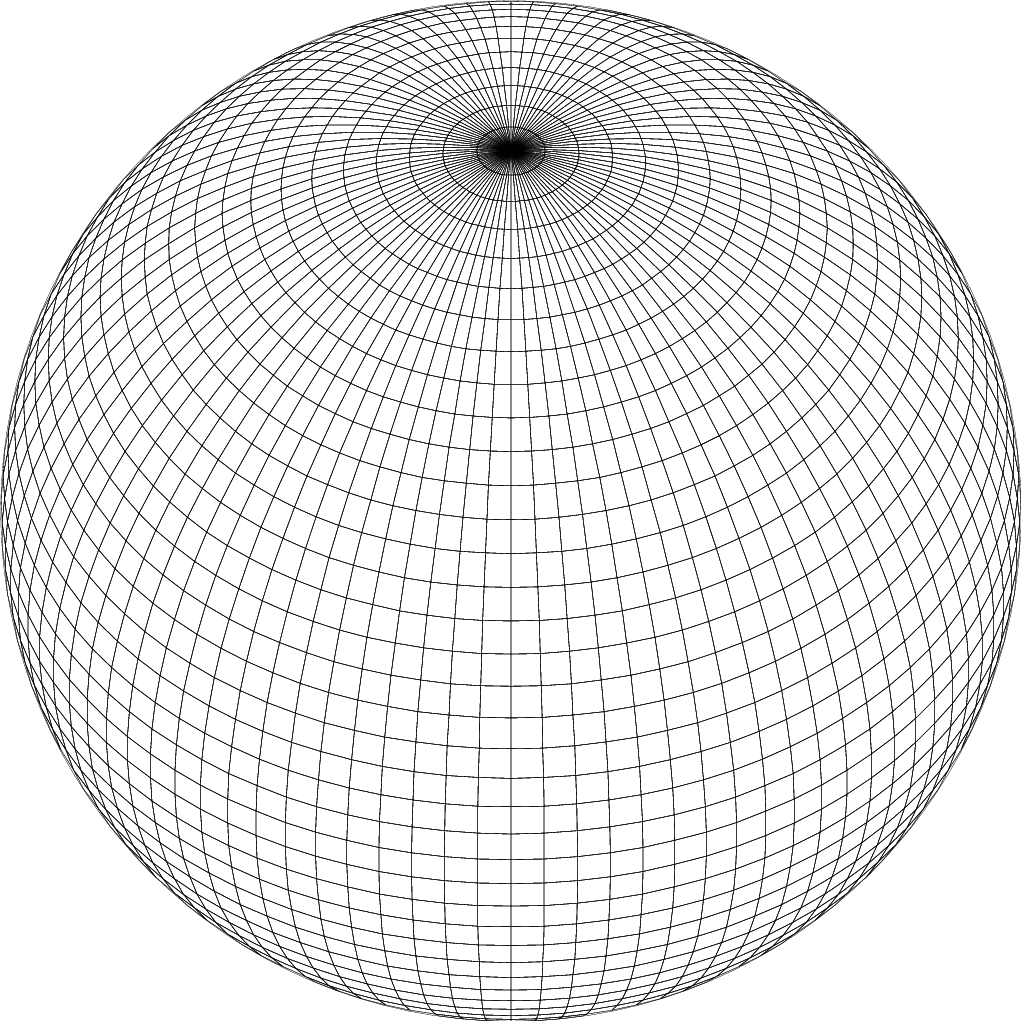
\includegraphics[width=2cm]{sphere-latlon}}; \node
      (B) [right=of A] {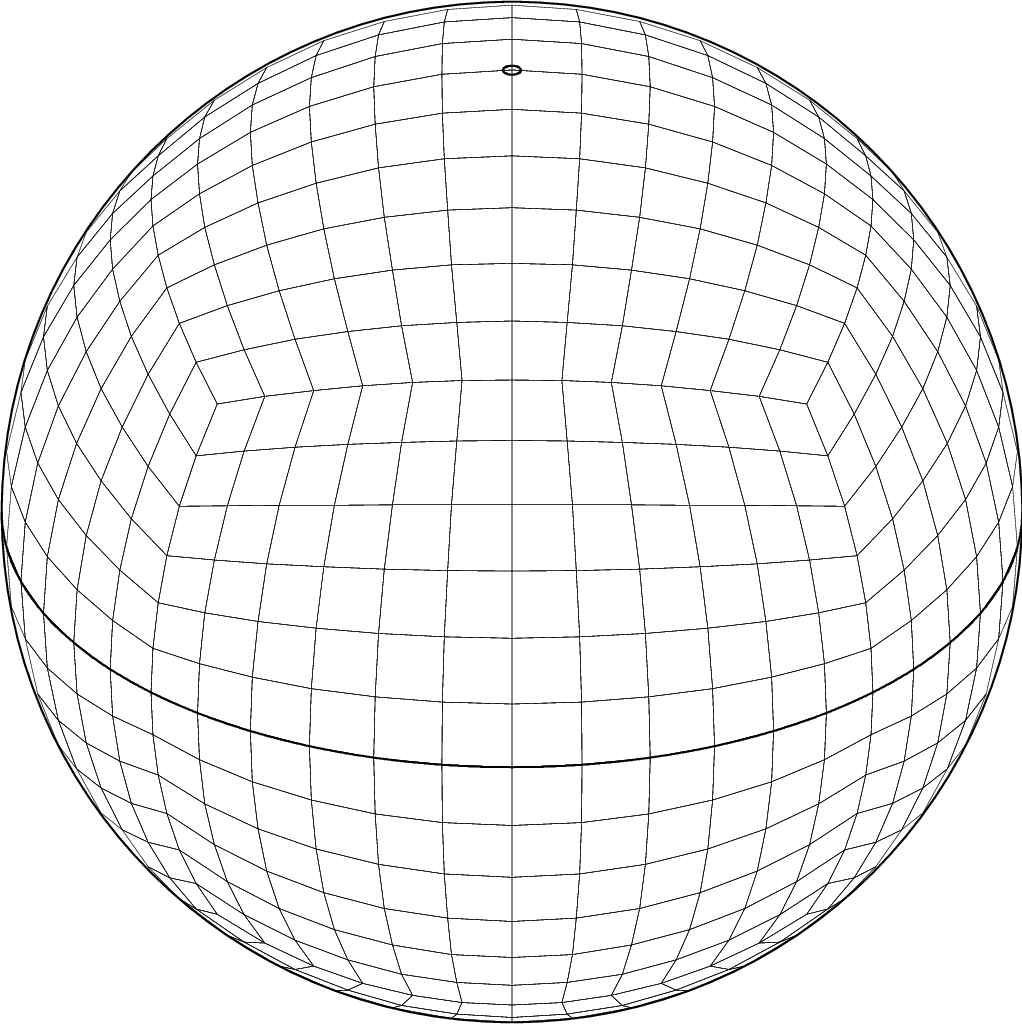
\includegraphics[width=2cm]{sphere-cubed}};
      \draw[-latex, very thick] (A)--(B);
    \end{tikzpicture}
  \end{center}
  Rules out the traditional staggered finite difference approaches.
  
  Instead, we use \emph{compatible finite elements} \parencite{Cotter:2012a}
\end{frame}

\begin{frame}
  \frametitle{Compatible FE}
  Choose a set of discrete spaces that match the properties of the
  continuous equations.  

  \begin{equation*}
    \W_0 \stackrel{\grad}{\longrightarrow}  \W_1  \stackrel{\curl}{\longrightarrow}  \W_2  \stackrel{\div}{\longrightarrow}  \W_3
  \end{equation*}

  Preserve vector calculus identities $\curl\grad = 0$,
  $\div\curl = 0$.

  Tensor product spaces on wedges

  \begin{center}
    \begin{tikzpicture}[scale=0.25]
      \node[thick, isosceles triangle, isosceles triangle apex
      angle=60, draw] (A) {};
    
      \node (B) [right=0.05cm of A] {$\otimes$};
    
      \node (C) [right=0.05cm of B, thick, rectangle, minimum
      width=0pt, inner sep=0pt, draw, minimum height=0.5cm] {};

      \draw[-latex, very thick] (C)++(0.5cm,0) -- +(2cm, 0);
      \begin{scope}[shift={($(C) + (3cm, -2cm)$)}]
        \draw[thick] (0,0) rectangle (4,4); \draw[thick] (0,0) --
        (1,1); \draw[thick] (4,0) -- (1,1); \draw[thick] (0,4) --
        (1,5); \draw[thick] (4,4) -- (1,5); \draw[thick] (1,1) --
        (1,5);
      \end{scope}
    \end{tikzpicture}
  \end{center}
\end{frame}

\begin{frame}
  \frametitle{Computational challenges}
  Implicit timestepping schemes result in an elliptic problem for
  pressure correction.

  Need a solver that is \emph{scalable} and \emph{fast}

  Large aspect ratio of domains is challenging for black box solvers.
\end{frame}

\section{Formulation}

\begin{frame}
  \frametitle{Linearised gravity wave}
  Linear system for velocity $\vec{u}$, pressure $p$ and buoyancy $b$.
  \begin{columns}
    \begin{column}{0.4\textwidth}
      \begin{align*}
        \label{eq:1}
        \ddt{\vec{u}} &= \nabla p + b \zhat, \\
        \ddt{p} &= -c^2 \nabla\cdot \vec{u}, \\
        \ddt{b} &= -N^2\vec{u}\cdot\zhat.\\
      \end{align*}
    \end{column}
    \begin{column}{0.6\textwidth}
      Domain $\Omega = S^2(R) \times [0, H]$.\\
      Enforce $\vec{u}\cdot \hat{\vec{n}} = 0$ at top and bottom.\\
      $R\approx 6000\textsf{km}$, $H\approx 80\textsf{km}$.
    \end{column}
  \end{columns}
\end{frame}

\begin{frame}
  \frametitle{Discretised system}
  After discretising in space and time we obtain a linear operator
\begin{equation*}
\begin{pmatrix}
  M_v & 
    -\frac{\Delta t}{2}D^T & 
    -\frac{\Delta t}{2}Q\\[1ex]
  \frac{\Delta t}{2}c^2D & M_p & 0\\[1ex]
  \frac{\Delta t}{2}N^2Q^T & 0 & M_b
\end{pmatrix}
\end{equation*}
with $M_{v,p,b}$ the velocity, pressure and buoyancy mass matrices
respectively, $D$ the weak derivative, and $Q$ the coupling between
velocity and buoyancy.
\end{frame}

\begin{frame}
  \frametitle{Preconditioning}
  Without mountains, buoyancy can be eliminated pointwise, with
  mountains the pointwise elimination is good in a preconditioner.  We
  focus on the velocity-pressure system
\begin{equation*}
\begin{pmatrix}
  M_v & -\frac{\Delta t}{2}D^T\\
  \frac{\Delta t}{2}c^2D & M_p\\
\end{pmatrix}
\end{equation*}

This is a discretisation of a sign-positive $H(\div)-L^2$ Helmholtz
equation.
\end{frame}

\begin{frame}[t]
  \frametitle{Options}
  \begin{columns}
    \begin{column}{0.5\textwidth}
      \begin{block}{Riesz map}
        Block diagonal preconditioner using the appropriate function
        space inner products
        \begin{equation*}
          \begin{pmatrix}
            (I - \grad \div)^{-1} & 0 \\
            0 & I\\
          \end{pmatrix}
        \end{equation*}
      \end{block}
      \begin{itemize}
      \item All operators sparse
      \item $H(\div)$ multigrid \parencite{Arnold:2000} is challenging
      \end{itemize}
    \end{column}
    \begin{column}{0.5\textwidth}
      \begin{block}{Schur complement}
        Block elimination and back substitution
        \begin{equation*}
          \begin{pmatrix}
            M_v^{-1} & 0 \\
            0 & S^{-1}\\
          \end{pmatrix}
        \end{equation*}
        where $S = M_p + \omega_c^2 D M_v^{-1} D^T$
      \end{block}
      \begin{itemize}
      \item $S$ is \emph{dense}, but elliptic
      \item invert using iterative method
      \item need preconditioner, $\tilde{S}$.
      \end{itemize}
    \end{column}
  \end{columns}
\end{frame}

\begin{frame}
  \frametitle{Approximating $S$}
  
\end{frame}
\section{Results}

\begin{frame}[allowframebreaks]
  \frametitle{Algorithmic performance}
  Convergence history

  CFL variation + time

  Mesh independence

\end{frame}

\begin{frame}
  \frametitle{}
  
\end{frame}

\begin{frame}
  \frametitle{Scaling}
  Weak scaling plots (time)
\end{frame}


\section{Concluding}

\begin{frame}
  \frametitle{Conclusions}
  Not so bad

  Programming this stuff is still painful

  Hybridisation?

  Auxiliary space \parencite{Hiptmair:2007} or $H(\div)$ multigrid?
\end{frame}

\begin{frame}[standout]
  
  Thanks!
  
\end{frame}
% \begin{frame}
%   \frametitle{Implementation}
%   Firedrake: hierarchy of extruded meshes

%   Banded matrix algebra and line smoothers with pyop2 -- foo
% \end{frame}

% \section{Results}

% \begin{frame}
%   \frametitle{Weak scaling}
  
% \end{frame}
\appendix
\begin{frame}[t, allowframebreaks]
  \frametitle{References}
  \printbibliography[heading=none]
\end{frame}
\end{document}
